\section{Ziel}
  Heutzutage ist es mit modernen Lasersystemen möglich ultrakurze Pulse im Bereich von wenigen Femtosekunden zu erzeugen und mit Hilfe dieser Prozesse mit Zeitskalen in der gleichen Größenordnung zu 
  untersuchen. Problematisch stellt sich dabei das Messen dieser ultrakurzen Pulse dar, weil die Messelektronik zu langsam arbeitet und nur Pulse bis zum niedrigen Nanosekundenbereich vermessen kann. In
  der Methode der Autokorrelation wird diese Limitierung umgangen, indem der fs-Puls mit sich selbst abgetastet wird und die Intensität bei jedem Abtastschritt über längere Zeit mit der vorhandenen 
  Elektronik gemessen werden kann. Solch ein Autokorrelator soll in diesem Versuch genutzt werden, um fs-Pulse sowie deren Verhalten beim Transmittieren durch Medien, wie Glas oder Silizium zu untersuchen.
    
\section{Theoretische Grundlagen}

  \subsection{Erzeugung ultrakurzer Pulse}
    Um Pulse mit Pulsdauern von wenigen Femtosekunden zu erzeugen, werden Laser, die Licht mit einer besonders großen Bandbreite erzeugen, mit der Technik des Mode-Locking kombiniert. Die große Bandbreite
    $\Delta\nu$ ist dabei notwendig, da die zeitliche Dauer des Pulses $\Delta\tau$ durch die Heisenberg'sche Unschärferelation in Form des Zeit-Bandbreite-Produkts 
    
    \begin{equation}
      \Delta\tau \cdot \Delta\nu = \text{const},
      \label{eqn:Heisenberg}
    \end{equation}
    
    das eine von der Pulsform abhängige Konstante besitzt, nach unten limitiert ist.    


    \subsubsection{Mode-Locking}
      In dem Resonator eines Laser können bis zu 100000 longitudinale Moden entstehen, die im Dauerstrich Laserbetrieb ohne feste Phasenbeziehung schwingen. Beim Mode-Locking wird versucht zwischen den 
      einzelnen Moden eine feste Phasenbeziehung zu erreichen, sodass es zu Interferenz zwischen den stehenden Wellen kommen kann. Dies führt, wie in Abbildung \ref{fig:Modelocking} a) zu sehen, zu einer 
      periodischen Wiederholung der Intensität mit der Durchlaufzeit durch den Resonator $T_C$. Zur Optimierung der Interferenz wird versucht die Phase aller Moden anzugleichen, sodass, wie in 
      Abbildung \ref{fig:Modelocking} b) dargestellt, letztendlich nur noch ein einzelnes ultrakurzes Wellenpaket durch den Resonator wandert und ausgekoppelt werden kann. Das Wellenpaket setzt sich also
      aus den stehenden Wellen der verschiedenen Frequenzen zusammen und kann als Fouriertransformation des Frequenzspektrums gesehen werden. Dies erklärt, dass die Menge der Moden und dementsprechend die 
      Bandbreite $\Delta\nu$ die minimal mögliche Pulsdauer $\Delta\tau_{\text{ML}}$ nach

      \begin{equation*}
        \Delta\tau_{\text{ML}} = \frac{2\pi}{\Delta\nu}
      \end{equation*}

      bestimmt. 
      Umgesetzt werden kann das Modelocking entweder durch die aktive Modulation, bei der zum Beispiel ein Shutter aktiv oszilliert, um längere Pulse abzuschwächen, oder durch passive Modulationen. In dem hier 
      genutzen System wird mit der Additiven Puls Modenkopplung eine passive Modulationsart genutzt. Diese beruht darauf, dass zunächst elliptisch polarisiertes Licht im Dauerstrichbetrieb durch ein Medium 
      läuft, dessen Brechungsindex linear mit der Intensität des Lichts ansteigt. Wenn eine zufällige Fluktuation der Laserintensität die Form eines Pulses annimmt, führt der nicht lineare Brechungsindex 
      zu einer Rotation der Ellipse, da die lineare Komponente der Ellipse mit der stärkeren Amplitude stärker zeitlich verzögert und damit die Phasenverschiebung der beiden zueinander verändert wird. Diese
      Rotation ist für das Zentrum des Pules größer als für die weniger intensiven Anteile. Dieser Puls durchläuft nun ein $\lambda/4$-Plättchen, das den Puls linear polarisiert und anschließend eine  
      $\lambda/2$-Plättchen, das den Puls um einen Winkel dreht. Dieser Winkel ergibt für die Pulse maximaler Intensität einen Polarisationswinkel, sodass der Anteil maximaler Amplitude durch einen 
      Polarized Beam-Splitter Cube (PBSC) transmittiert wird. Für Pulsanteile geringerer Intensität ist der finale Winkel nicht optimal, sodass diese Anteile unterdrückt und effektiv abgeschnitten werden. Nach
      Transmission durch den PBSC wird der Puls erneut aus einer Kombination von einem $\lambda/2$- und $\lambda/4$-Plättchen elliptisch polarisiert. Die so erreichbaren Pulsdauern liegen im Bereich von 
      \SI{100}{\femto\second}, sofern der Strahlungsübergang des Lasers eine genügend große Linienbreite und somit viele lasefähige Moden besitzt. 

      \FloatBarrier
      \begin{figure}[h]
        \centering
        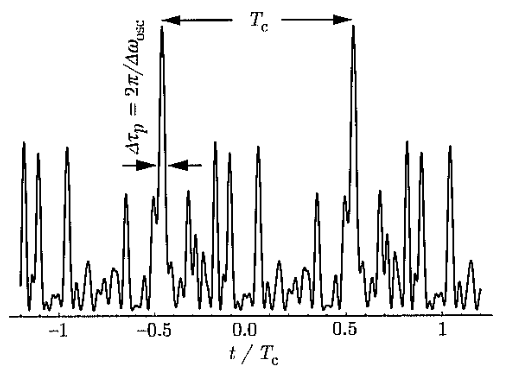
\includegraphics[width = 0.44\textwidth]{pictures/ML_phase_const.png}
        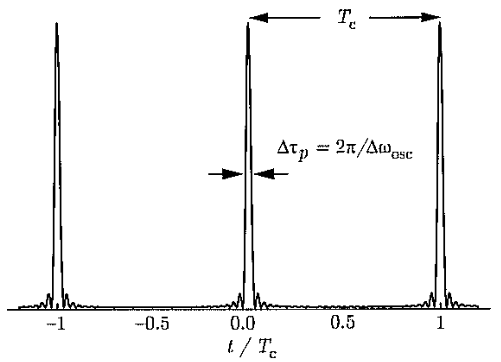
\includegraphics[width = 0.44\textwidth]{pictures/ML_phase_gleich.png}
        \caption{a) Zeitlicher Verlauf der Intensität des Laser bei Überlagerung der Moden mit fester Phasenbeziehung. b)Zeitlicher Verlauf der Intensität, wenn die Moden alle die gleiche Phase besitzen. Entnommen aus \cite{hooker_laser_2010}}
        \label{fig:Modelocking}
      \end{figure}
      \FloatBarrier
      
    \newpage
    \subsubsection{fs-Laser}

      Das in diesem Versuch genutzte und in Abbildung \ref{fig:Laser} dargestellte Lasersystem setzt sich aus einem Faserlaser zusammen, der mit einem Ringresonator in Kombination mit Verzögerungsplättchen 
      und eines PBSCs, einer undotierten Faser mit negativer Group-Velocity-Dispersion (GVD), einer dotierten Faser mit positiver GVD und weiteren Verzögerungsplättchen und Silizium Prismen zur Erzeugung von
      ultrakurzen Pulsen genutzt wird. 

      \FloatBarrier
      \begin{figure}[h]
        \centering
        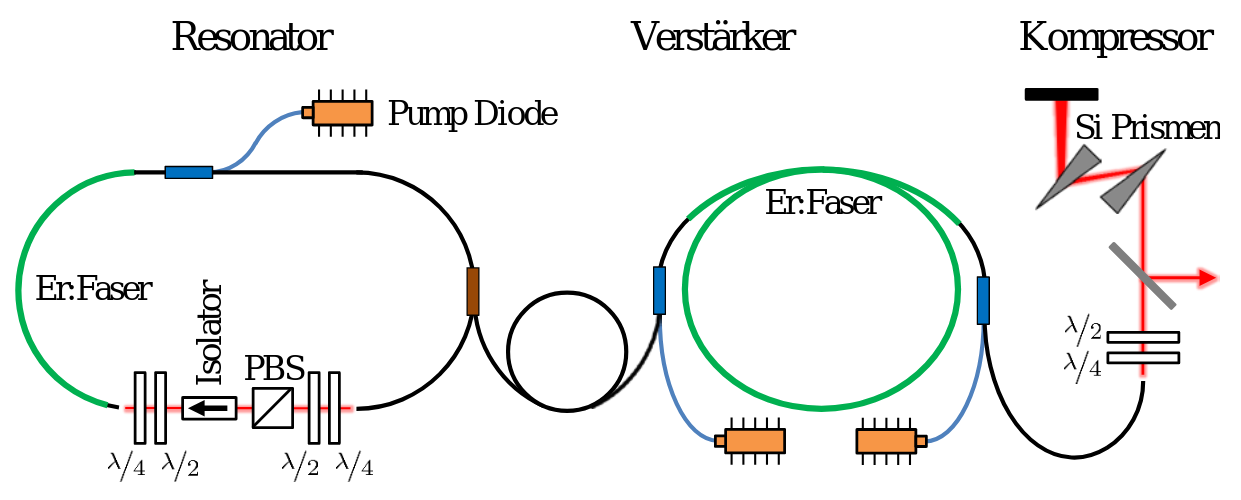
\includegraphics[width = 0.9\textwidth]{pictures/Laser.png}
        \caption{Aufbau des Laser zur Erzeugung von ultrakurzen Pulsen. Entnommen aus \cite{toptica}}
        \label{fig:Laser}
      \end{figure}
      \FloatBarrier

      Zur Erzeugung der primären Strahlung wird eine Quarzglas-Glasfaser genutzt, deren innerer Kern mit Er$^{3+}$-Ionen dotiert ist und als aktives Medium fungiert. Ein infraroter Laser mit einer Wellenlänge von 
      \SI{980}{\nano\metre} regt die Er$^{3+}$-Ionen in den höchsten Zustand eines Drei-Niveau-Systems an, dessen Übergang in den Grundzustand dipolverboten ist. Daher kann schnell eine Besetzungsinversion
      erreicht werden und durch Übergang in den zweithöchsten Zustand anschließend ein strahlender Übergang stattfinden. Dieser emittiert bei einer zentralen Wellenlänge von \SI{1550}{\nano\metre} und besitzt 
      eine große Bandbreite, da die zugehörigen Zustände durch die Elektron-Phonon-Wechselwirkung des dotierten inneren Kerns mit dem undotierten Quarzglas der äußeren Schicht stark verbreitert sind.
      
      Die so entstehende Strahlung befindet sich zunächst im Dauerstrichbetrieb und wird wie zuvor beschrieben über die Additiven Puls Modenkopplung im Ringresonator transformiert. Anschließend werden diese 
      Pulse ausgekoppelt und durch eine Faser mit negativer GVD transmittiert. Die GVD steckt in der Taylorentwicklung der Dispersion um die zentrale Frequenz $\omega_0$
      
      \begin{equation}
        \phi(\omega) = \phi_0 + \text{GD} \cdot \left(\omega-\omega_0\right) + \frac{1}{2} \text{GVD} \cdot \left(\omega-\omega_0\right)^2 \,,
      \end{equation}
      
      die die Abhängigkeit des Wellenvektors beziehungsweise der Phase $\phi$ von der instantanen Kreisfrequenz $\omega$ angibt. Die Gruppenverzögerung (GD) gibt an, wie lange Frequenzanteile eines Pulses
      benötigen, um durch ein Medium zu propagieren. Die GVD wiederum beschreibt, wie die GD von der Frequenz des Lichts abhängt. Wie in Abbildung \ref{fig:Dispersion} dargestellt, führt die Dispersion zu
      einer Erhöhung der Pulsdauer

      \begin{equation}
        \Delta\tau_{\text{neu}} = \sqrt{1 + \left(\frac{4\ln\left(2\right)\cdot \text{GVD}}{\Delta\tau_{\text{alt}}^2}\right)^2} \, ,
      \end{equation}
      
      die für hohe GVD und kurze Pulsdauern $\Delta\tau_{\text{alt}}$ maximal wird.
      Bei normaler Dispersion laufen höhere Frequenzen schneller und bei anormaler Dispersion laufen niedrigere schneller. Dies führt wie in Abbildung \ref{fig:Dispersion} zu
      erkennen zu einem sogennaten Chirp, der die Änderung der Frequenz eines Pulses entlang seiner Zeitskala beschreibt. Zusätzlich tritt in dieser Faser auch der nicht-lineare Effekt der 
      Selbstphasenmodulation auf, der die Bandbreite des Pulses bei Propagation durch ein nicht lineares Medium wie Quarzglas erhöht.
  

      \FloatBarrier
      \begin{figure}[h]
        \centering
        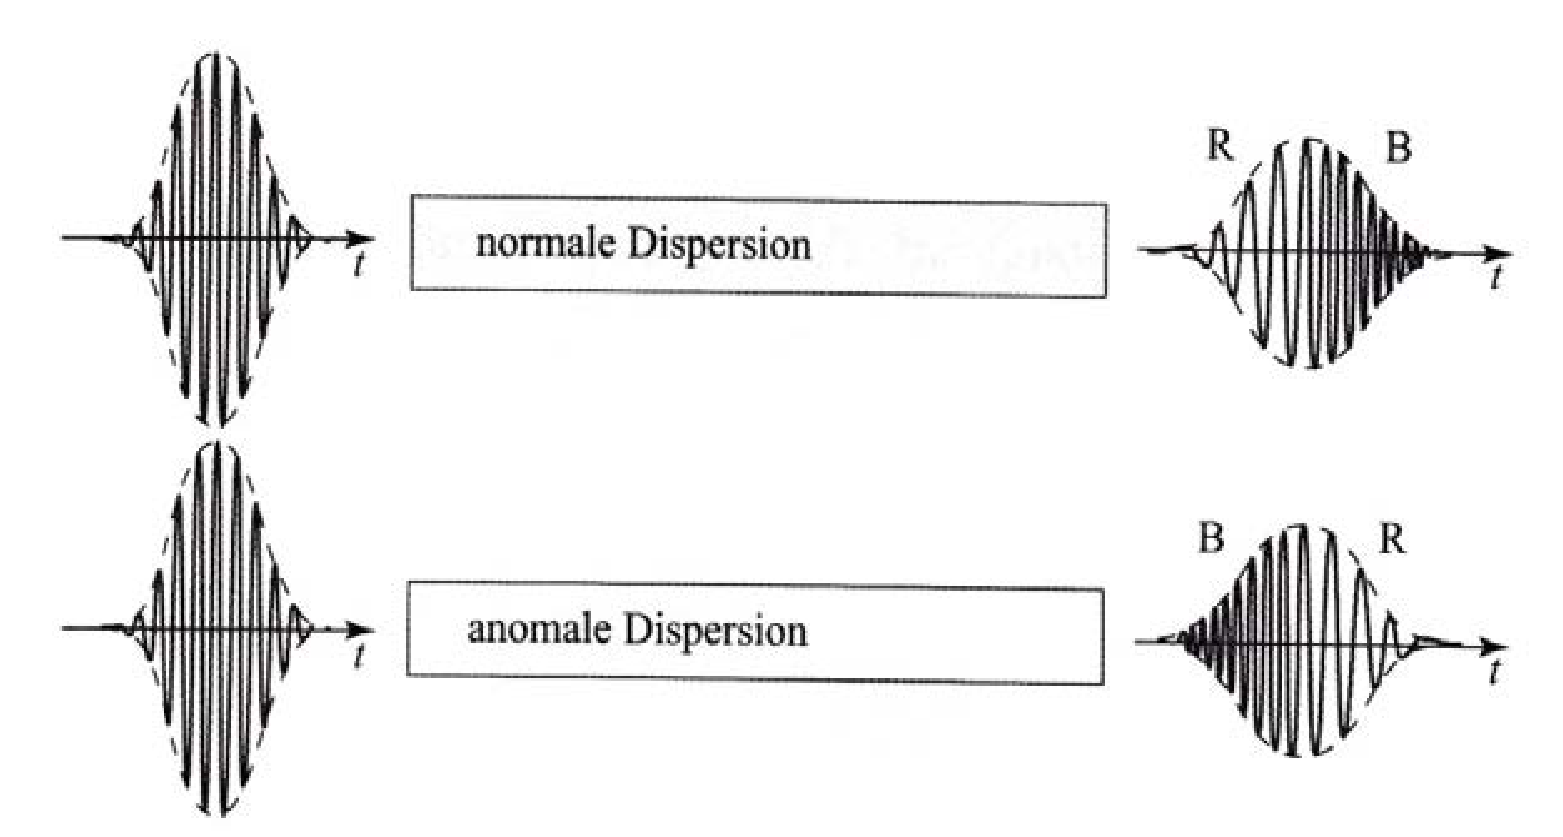
\includegraphics[width = 0.77\textwidth]{pictures/Dispersion.png}
        \caption{Aufbau des Laser zur Erzeugung von ultrakurzen Pulsen. Entnommen aus \cite{jostmeier_koharente_2012}}
        \label{fig:Dispersion}
      \end{figure}
      \FloatBarrier


      Der nun bezüglich seiner Bandbreite und Dauer gestreckte Puls, wird in eine mit Er$^{3+}$-Ionen dotierte und gepumpte Faser eingekoppelt, deren GVD postiv ist. Die hier auftretende Dispersion 
      kompensiert zum einen den zuvor entstandenen Chirp und kann zusätzlich den Puls auf nun noch kürzere Dauern komprimieren, da die Limitierung durch die erhöhte Bandbreite gesenkt wird. Die
      Kompression funktioniert über das Aufholen der in der undotierten Faser noch langsammeren Frequenzanteile auf die zuvor schnelleren aufgrund der umgekehrten GVD. Die so komprimierten Pulse sind 
      quasi chirpfrei und werden nach horizontaler Polarisierung durch eine Kombination eines $\lambda/2$- und $\lambda/4$-Plättchens noch durch zwei Silizium-Prismen bezüglich ihrer Pulsdauer und ihres 
      Chirps feinjustiert. Letztendlich wird so ein gepulster Laserbetrieb bei einer zentralen Wellenlänge von \SI{1550}{\nano\metre} und einer Pulsdauer von circa \SI{100}{\femto\second} bei gaußförmiger 
      Pulsform erreicht.
      
    
    \subsection{Vermessung ultrakurzer Pulse}
      \subsubsection{Autokorrelation}
        Bei der Autokorrelation wird, wie in der Einleitung beschrieben ein Laserpuls mit einer Kopie von sich selbst abgetastet, sodass ein zeitliches Intensitätsprofil dessen erstellt wird. Da der Abtastpuls
        so immer in der Größenordnung des zu vermessenden Pulses liegt, können so auch ultrakurze Pulse vermessen werden. Um die Autokorrelation vermessen zu können, müssen die beiden Pulse räumlich und
        zeitlich überlagert werden. Bei interferometrischen Autokorrelatoren kommt es dann zu Interferenz zwischen den einzelnen Pulsen, aus der Informationen über die Länge des Pulses und dessen Chirp 
        gewonnen werden kann. Bei der in diesem Versuch genutzen Intensitätsautokorrelation werden die Pulse in einem nicht linearen Medium überlagert und der Effekt der Summenfrequenzerzeugung genutzt, 
        um Informationen über die Pulslänge aber nicht den Chirp zu erhalten.  


      \subsubsection{Summenfrequenzerzeugung}

        Beim Prozess der Summenfrequenzerzeugung (\textit{Sum Frequency Generation}, SFG) generieren zwei Photonen in einem nicht-linearen Kristall ein drittes Photon. In der Wellenbeschreibung des Lichts 
        entspricht dies zwei elektrischen Feldern einfallender Strahlen, die einen dritten Strahl erzeugen, dessen elektrisches Feld mit der Summe der Frequenzen der ursprünglichen Felder schwingt. Zur 
        Erklärung dieses Phänomens muss die durch Licht induzierte Polarisation eines Mediums betrachtet werden. Da die SFG ein nicht-linearer Effekt zweiter Ordnung ist, wird die Potenzreihe der Polarisation 
        $P$ auf die ersten beiden Summanden beschränkt und skalar betrachtet
        %
        \begin{equation*}
            P = \varepsilon_0 \left( \chi^{\left( 1 \right)}  E + \chi^{\left( 2 \right)}  E^2 \right) ,
        \end{equation*}
        %
        sodass zwischen einem linearen und einem nicht-linearen Summanden unterschieden werden kann. Zusätzlich erfordert die quadratische Abhängigkeit von dem elektrischen Feld, dass das nicht-lineare Medium 
        nicht zentrosymmetrisch ist, weil der quadratische Term dann keinen Beitrag liefern würde. Als Ansatz der elektrischen Felder der einfallenden Photonen mit den Amplituden $A_1$ und $A_2$ wird eine 
        Summe gewählt
        %
        \begin{equation*}
            E(t) = A_1  \cos\left(\omega_1 t - \vec{k}_1 \cdot \vec{r}\right) + A_2  \cos\left(\omega_2 t - \vec{k}_2 \cdot \vec{r}\right),
        \end{equation*}
        %
        die aufgrund des Skalarprodukts zwischen dem Wellenvektor $\vec{k}_{\text{i}}$ und dem Ortsvektor $\vec{r}$ auch die Ausbreitungsrichtung der beiden Photonen berücksichtigt. Wird dieser Ansatz in die 
        Polarisation eingesetzt, ergeben sich als lineare Reaktion der Polarisation zwei Schwingungen, die mit den Fundamentalfrequenzen $\omega_{1,2}$ schwingen. Aufgrund der quadratischen Antwort entsteht 
        neben hier vernachlässigten Summanden ein Beitrag 
        %
        \begin{equation*}
            P_{\text{SFG}} = \varepsilon_0  \chi^{(2)}  A_1 A_2  \cos\left( \left(\omega_1 + \omega_2\right) t - \left( \vec{k}_1 + \vec{k}_2 \right) \cdot \vec{r} \right) ,
        \end{equation*}
        %
        der eine Schwingung mit der Frequenz $\omega_3 = \omega_1 + \omega_2$ beschreibt. Dies entspricht der der SFG zugrundeliegenden Polarisation 
        $P_{\text{SFG}}$, deren Amplitude dem Produkt der fundamentalen Schwingungsamplituden entspricht. Aufgrund des proportionalen Zusammenhangs zwischen Polarisation und elektrischem Feld erzeugt 
        $P_{\text{SFG}}$ eine zusätzliche elektrische Schwingung. Für den Fall zwei gleicher Pulser entspricht die SFG der Erzeugung der zweiten Harmonischen.

      \subsubsection{Intensitätsautokorrelation}  
      \label{sec:AK47}
        Bei der Intensitätsautokorrelation wird der zu vermessenden Laserpulses zunächst, wie in Abbildung \ref{fig:autokorrelator} dargestellt, über einen Strahlteiler in zwei Pulse aufgeteilt. 
        Der optische Weg $\Delta x$ einer der Pulse kann verändert werden, da dieser an Spiegeln, die auf einer mechanischen Schiebeplattform befestigt sind, reflektiert wird. Auf diese Weise lässt sich 
        ein zeitlicher Versatz $\tau=\frac{2\Delta x}{\text{c}}$ zwischen den beiden Pulsen erzeugen. Nachdem einer der Pulse die sogenannte Verzögerungsstrecke durchlaufen hat, werden beide Pulse in ein 
        nicht-lineares Medium, hier ein 
        $\beta$-Bariumborat(BBO)-Kristall, fokussiert, der zur Erzeugung von zweiten Harmonischen geeignet ist. Dabei interferieren die beiden Pulse und erzeugen zum einen jeweils ihre eigene zweite Harmonische 
        (\textit{Second Harmonic Generation}, SHG) und bei zeitlichem sowie räumlichem Überlapp zusätzlich einen weiteren Puls, der aus der SFG der beiden Pulse entsteht. Da die beiden einfallenden Pulse nicht 
        kollinear verlaufen, lassen sich die beiden zweiten Harmonischen durch Blenden unterdrücken und nur das SFG-Signal durch eine Photodiode detektieren. Photodioden sind Dioden, die in Sperrichtung und 
        bei möglichst keiner Bias-Spannung betrieben werden. Auf diese Weise lässt sich ein zur einstrahlenden Intensität linearer Strom mit geringem Untergrund messen, sofern die Photonenenergie genügt, um
        Elektronen des Diodenmaterials aus dem Valenz- in das Leitungsband anzuheben.  
        %
        \FloatBarrier
        \begin{figure}[h]
          \centering
          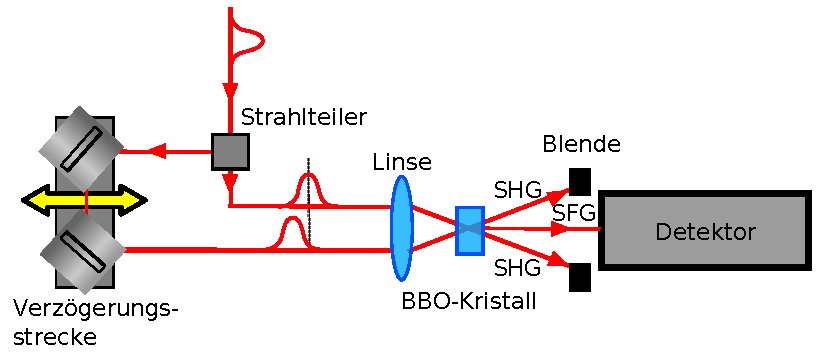
\includegraphics[width = 0.9\textwidth]{pictures/autokorrelator.pdf}
          \caption{Typischer Aufbau zur Vermessung ultrakurzen Pulsen mittels Intensitätsautokorrelation.}
          \label{fig:autokorrelator}
        \end{figure}
        \FloatBarrier
        %
        Das SFG-Signal $S_{\text{SFG}}$
        %
        \begin{equation}
            S_{\text{SFG}} = \int_{-\infty}^{\infty} \left(E^2 (t)  E^2 (t-\tau)\right) \text{d}t ,
            \label{eqn:autocor}
        \end{equation}
        %
        das sich in Abhängigkeit des zeitlichen Versatzes $\tau$ zwischen den beiden Pulsen ändert, wird in der Autokorrelation gemessen. Es handelt sich dabei um die mathematische Faltung des Pulses $E(t)$ 
        mit seinem zeitlich versetzten Abbild $E(t - \tau)$. Dies wird als Intensitätsautokorrelation bezeichnet. Die Änderung des optischen Weges durch die Verzögerungsstrecke erlaubt das Messens des Signals 
        für unterschiedliche $\tau$. Dies entspricht dem Abtasten des Pulses mit sich selbst. Aus der resultierenden Halbwertsbreite der Intensitätsautokorrelation lässt sich über einen Faktor 
        $C^{\text{Pulsform}}$, der für verschiedene Pulsformen variiert, mittels 
        %
        \begin{equation*}
            \tau_{\text{FWHM}}^{\text{Pulsform}} = \frac{1}{C^{\text{Pulsform}}} \cdot \tau_{\text{FWHM}}^{\text{Autokorrelation}}
        \end{equation*}
        %
        leicht die zeitliche Halbwertsbreite dieses Pulses bestimmen. Dieses Konzept gibt Rückschlüsse auf die zeitliche Pulsdauer. 
        Für einen gauß´schen Puls der Dauer $\Delta \tau$ der Form

        \begin{equation}
          \text{I}(t) \propto \exp\left(-4\ln(2)\left(\frac{t}{\Delta \tau}\right)^2\right)
          \label{eqn:IntGauss}
        \end{equation}

        ergibt das Einsetzen in Gleichung \ref{eqn:autocor} folgenden Zusammenhang zwischen der zeitlichen Halbwertsbreite der Autokorrelation und der Pulsdauer:

        \begin{equation*}
          \Delta\tau_{\text{FWHM}}^{\text{Pulsform}} = \frac{1}{\sqrt{2}} \cdot \Delta\tau_{\text{FWHM}}^{\text{Autokorrelation}}
          \label{eqn:tautau}
        \end{equation*}
        
        Um bei der Messung das Hintergrundrauschen zu unterdrücken, kann das 
        einfallende Licht durch einen Chopper mit festgelegter Frequenz moduliert werden. Das Signal der Photodiode wird mit dem Signal des Choppers moduliert und über einen Lock-In-Filter integriert.


